\section{Пример добавления в документ рисунка из файла, созданного сторонней программой}
\sectionmark{Пример добавления в документ рисунка из файла}

\subsection{Один рисунок}

На рисунке~\ref{p:func_in2_1} приведена функциональная 
схема измерителя напряжения ИН2. В книге \cite{gussens} можно найти дополнительные сведения по включению рисунков в документ.


\begin{figure}[!h]
  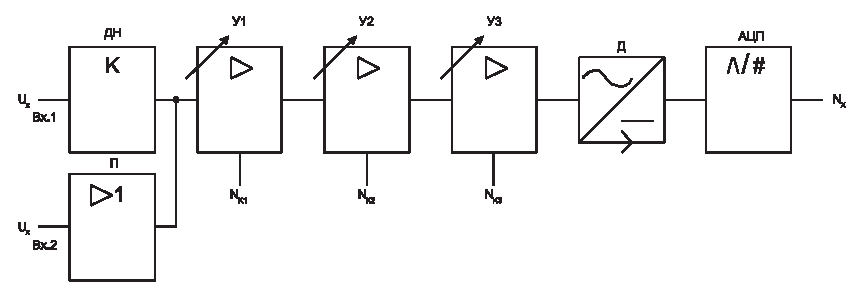
\includegraphics[width=1\textwidth]{./about/func_in}
  \caption{Функциональная схема измерителя напряжения ИН2, необходимая для демонстрации возможностей включения рисунков и корректного переноса подрисуночной подписи} \label{p:func_in2_1}
\end{figure}


\subsection{Два рисунка в ряд }

\begin{figure}[H]
\begin{minipage}[h]{0.49\linewidth}
\center{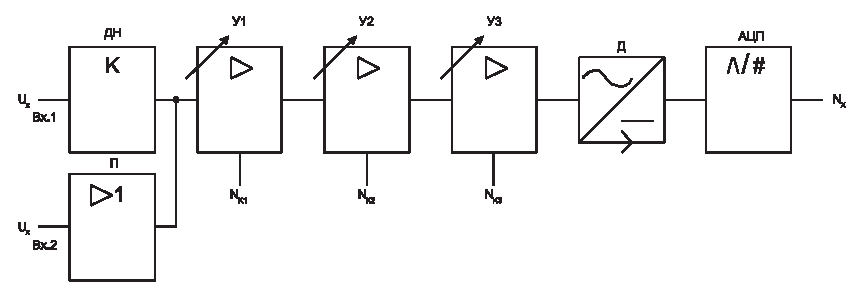
\includegraphics[width=0.7\linewidth]{./about/func_in} \\ а)}
\end{minipage}
\hfill
\begin{minipage}[h]{0.49\linewidth}
\center{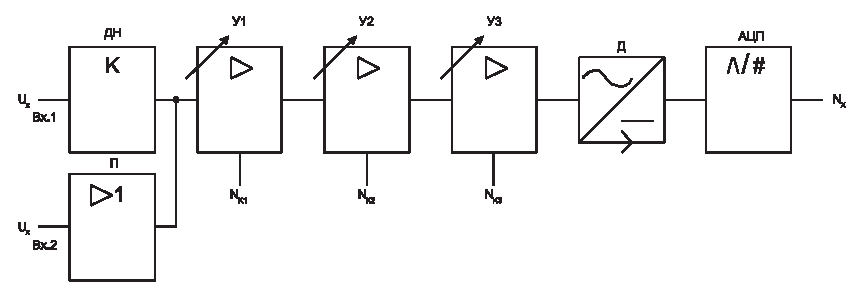
\includegraphics[width=0.7\linewidth]{./about/func_in} \\ б)}
\end{minipage}
\caption{Зависимость сигнала от шума для данных.}
\label{ris:image1}
\end{figure}



\newpage
\subsection{Два рисунка в ряд с разными подписями}


\begin{figure}[H]
\begin{center}
  \captionsetup{width=60mm}%
\begin{minipage}[h]{0.4\linewidth}
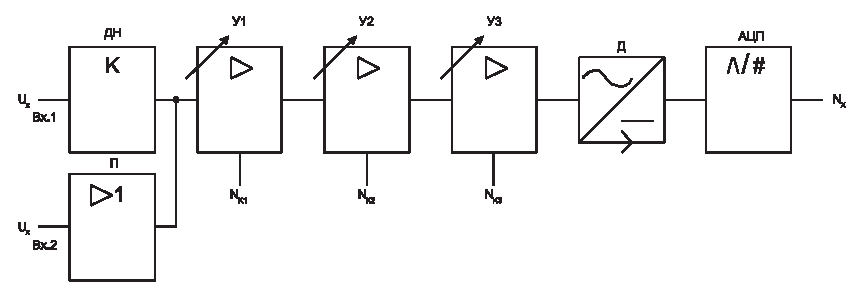
\includegraphics[width=1\linewidth]{./about/func_in}
\caption{Исходное изображение.} %% подпись к рисунку
\label{ris:experimoriginal} %% метка рисунка для ссылки на него
\end{minipage}
\hfill
\begin{minipage}[h]{0.4\linewidth}
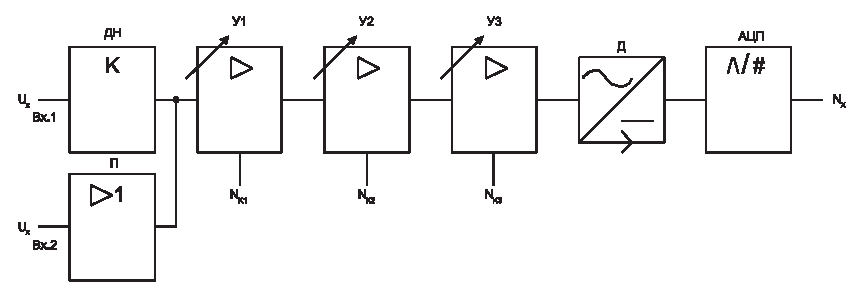
\includegraphics[width=1\linewidth]{./about/func_in}
\caption{Закодированное изображение.}
\label{ris:experimcoded}
\end{minipage}
\end{center}
\end{figure}



\begin{figure}[H]
\begin{center}
  \captionsetup{width=50mm,
      %margin={250mm,-250mm}
      }%
\begin{minipage}[h]{0.3\linewidth}
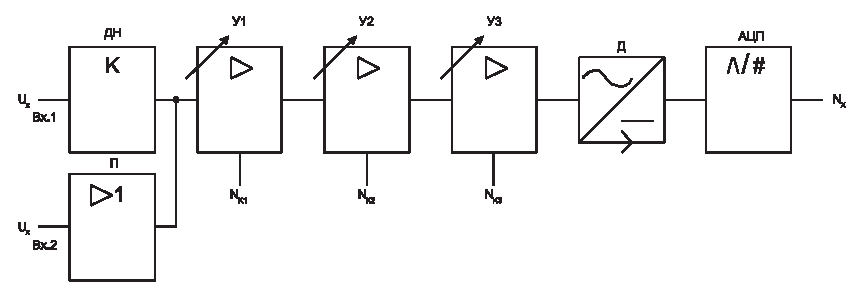
\includegraphics[width=1\linewidth]{./about/func_in}
\caption{} %% подпись к рисунку
\label{ris:expe1} %% метка рисунка для ссылки на него
\end{minipage}
\hfill
\begin{minipage}[h]{0.3\linewidth}
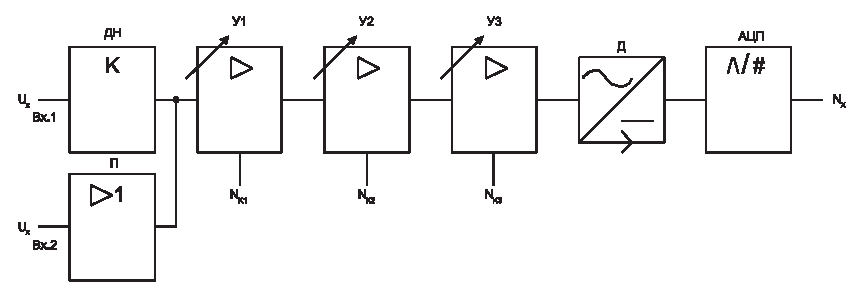
\includegraphics[width=1\linewidth]{./about/func_in}
\caption{}
\label{ris:expe2}
\end{minipage}
\hfill
\begin{minipage}[h]{0.3\linewidth}
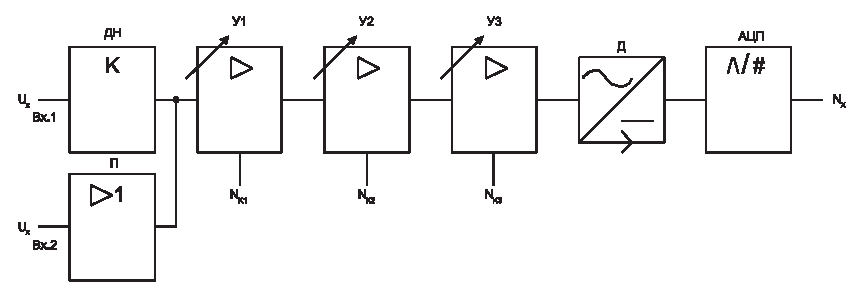
\includegraphics[width=1\linewidth]{./about/func_in}
\caption{}
\label{ris:expe3}
\end{minipage}
\end{center}
\end{figure}






%\subsection{Рисунок, сделанный в LaTeXDraw}

%\begin{pspicture}(0,-1.91)(6.3,1.91)
%\psframe[linewidth=0.04](3.44,0.77)(0.92,-0.77)
%\psframe[linewidth=0.04](4.24,1.07)(2.4,0.09)
%\psline[linewidth=0.04cm](2.76,1.53)(4.06,-0.09)
%\psline[linewidth=0.04cm](6.28,1.19)(0.02,-1.89)
%\psline[linewidth=0.04cm](5.42,1.89)(5.28,-0.07)
%\end{pspicture}





\subsection{Рисунок, сделанный в Inkscape}

\begin{figure}[H] \centering
\input ./about/inkscape/drawing1.tex
\caption{Рисунок, сделанный в Inkscape. Включен в документ как файл с *.tex-кодом (довольно громоздким), правильно отрисовываются русские буквы, даже растянутые}
\label{ris:image1_ink}
\end{figure}


\subsection{Рисунок, сделанный в Dia}

\begin{figure}[H] \centering
\input ./about/dia/drawing1.tex
\caption{Рисунок, сделанный в Dia. Включен в документ как файл с *.tex-кодом (по сравнению с Inkscape довольно компактный), русские буквы отрисовываются основным шрифтом документа, стрелки на концах линий не так масштабируются}
\label{ris:image1_dia}
\end{figure}



\begin{figure}[H] \centering \fontspec[Scale=2.0]{Times New Roman}
\input ./about/dia/drawing1.tex
\caption{Рисунок, сделанный в Dia. Увеличили шрифт текста прямо в LaTeX}
\label{ris:image1_dia}
\end{figure}






